\chapter{Implementasi dan Pengujian}
\label{chap:implementasi}

\section{Implementasi}

\subsection{Lingkungan Implementasi}
Implementasi perangkat lunak ini dilakukan di komputer penulis dengan spesifikasi sebagai berikut:

\begin{enumerate}
    \item \textit{Processor}: Intel Core i7-9750H
    \item \textit{Random Access Memory} (RAM): 16GB DDR4
    \item \textit{Graphics Processing Unit} (GPU): NVIDIA GeForce GTX 1650
    \item \textit{Storage}: 512 GB SSD
    \item Sistem Operasi: Windows 11 
    \item Versi \textit{node}: v14.17.6
    \item Versi \textit{npm}: 6.14.15
\end{enumerate}

\subsection{Hasil Implementasi}
Hasil implementasi aplikasi VisKur berupa tampilan visualisasi dalam bentuk \textit{Network} dan \textit{Timeline}. 

\begin{itemize}
    \item Contoh hasil visualisasi \textit{Network} dapat dilihat pada Gambar \ref{fig:gambarNetwork1} dan Gambar \ref{fig:gambarNetwork2}.
    
    \begin{figure}[H]
        \centering
        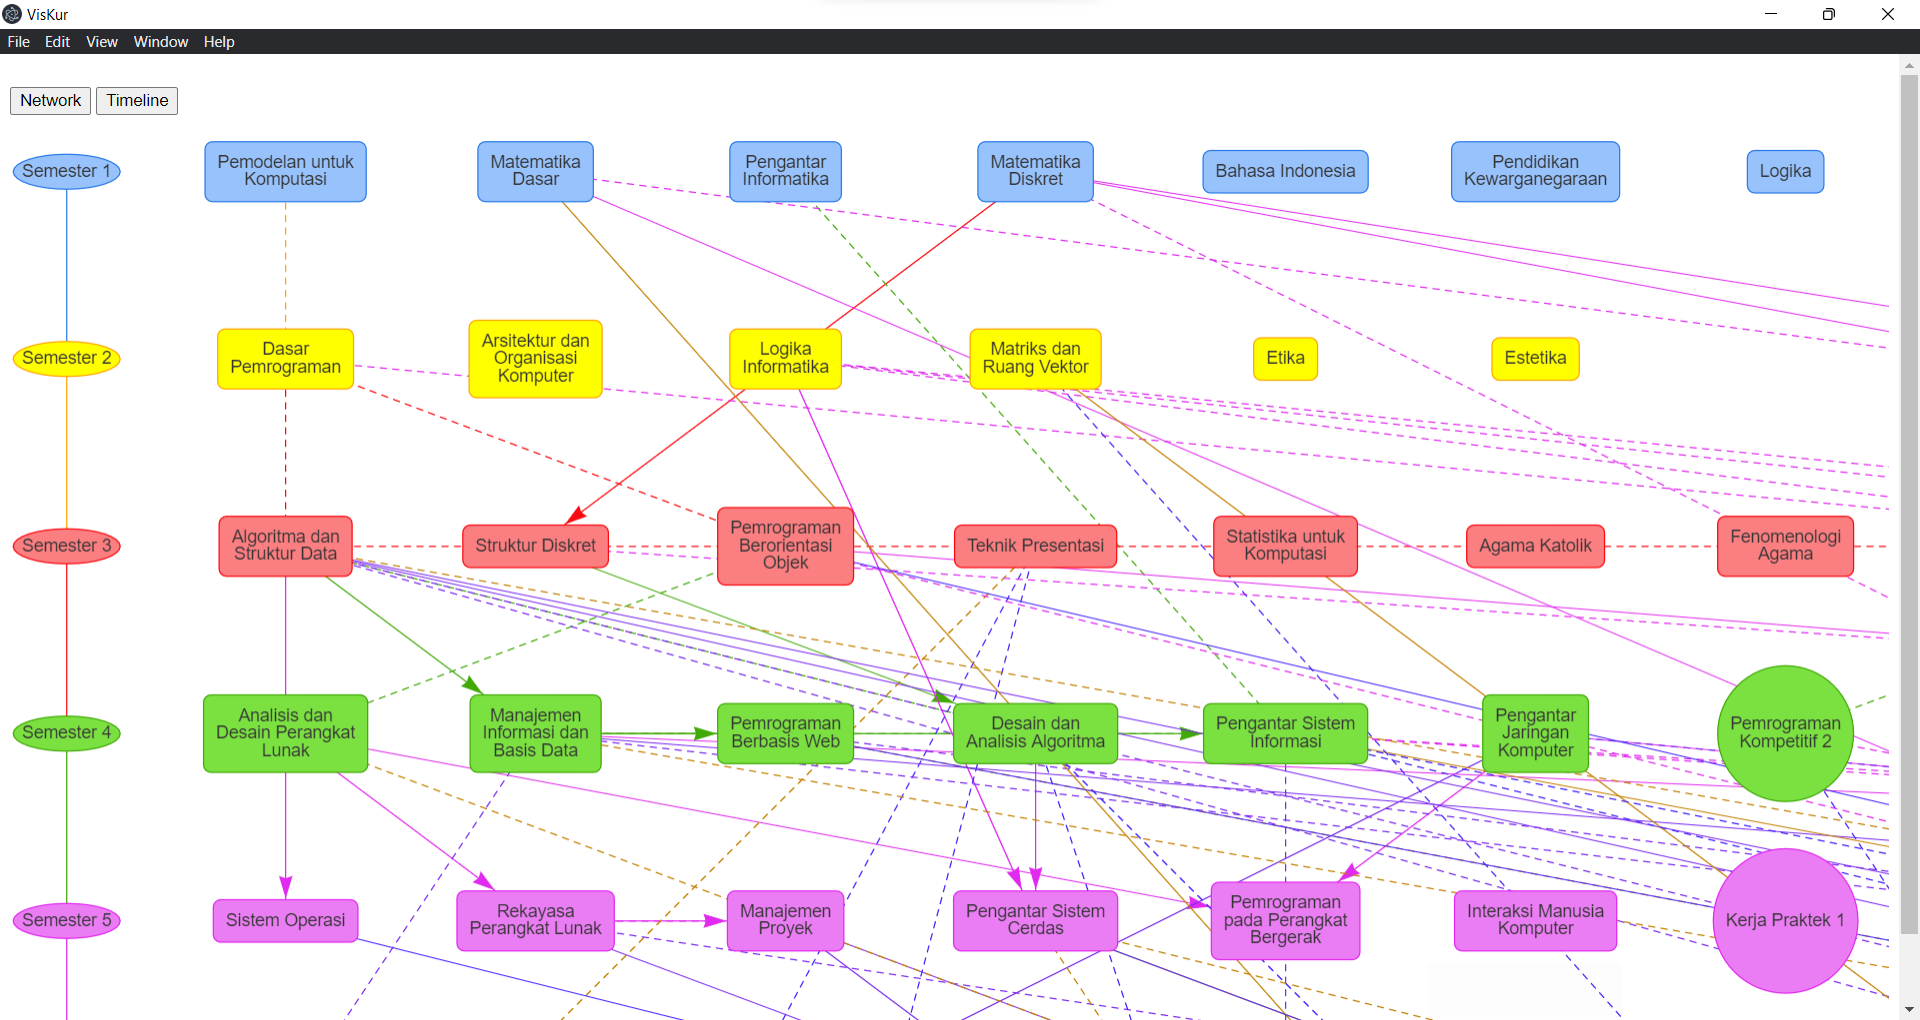
\includegraphics[width=12cm, height=8cm]{Gambar/Network1.png}
        \caption{Hasil visualisasi \textit{Network}1}
        \label{fig:gambarNetwork1}
    \end{figure}
    
    \begin{figure}[H]
        \centering
        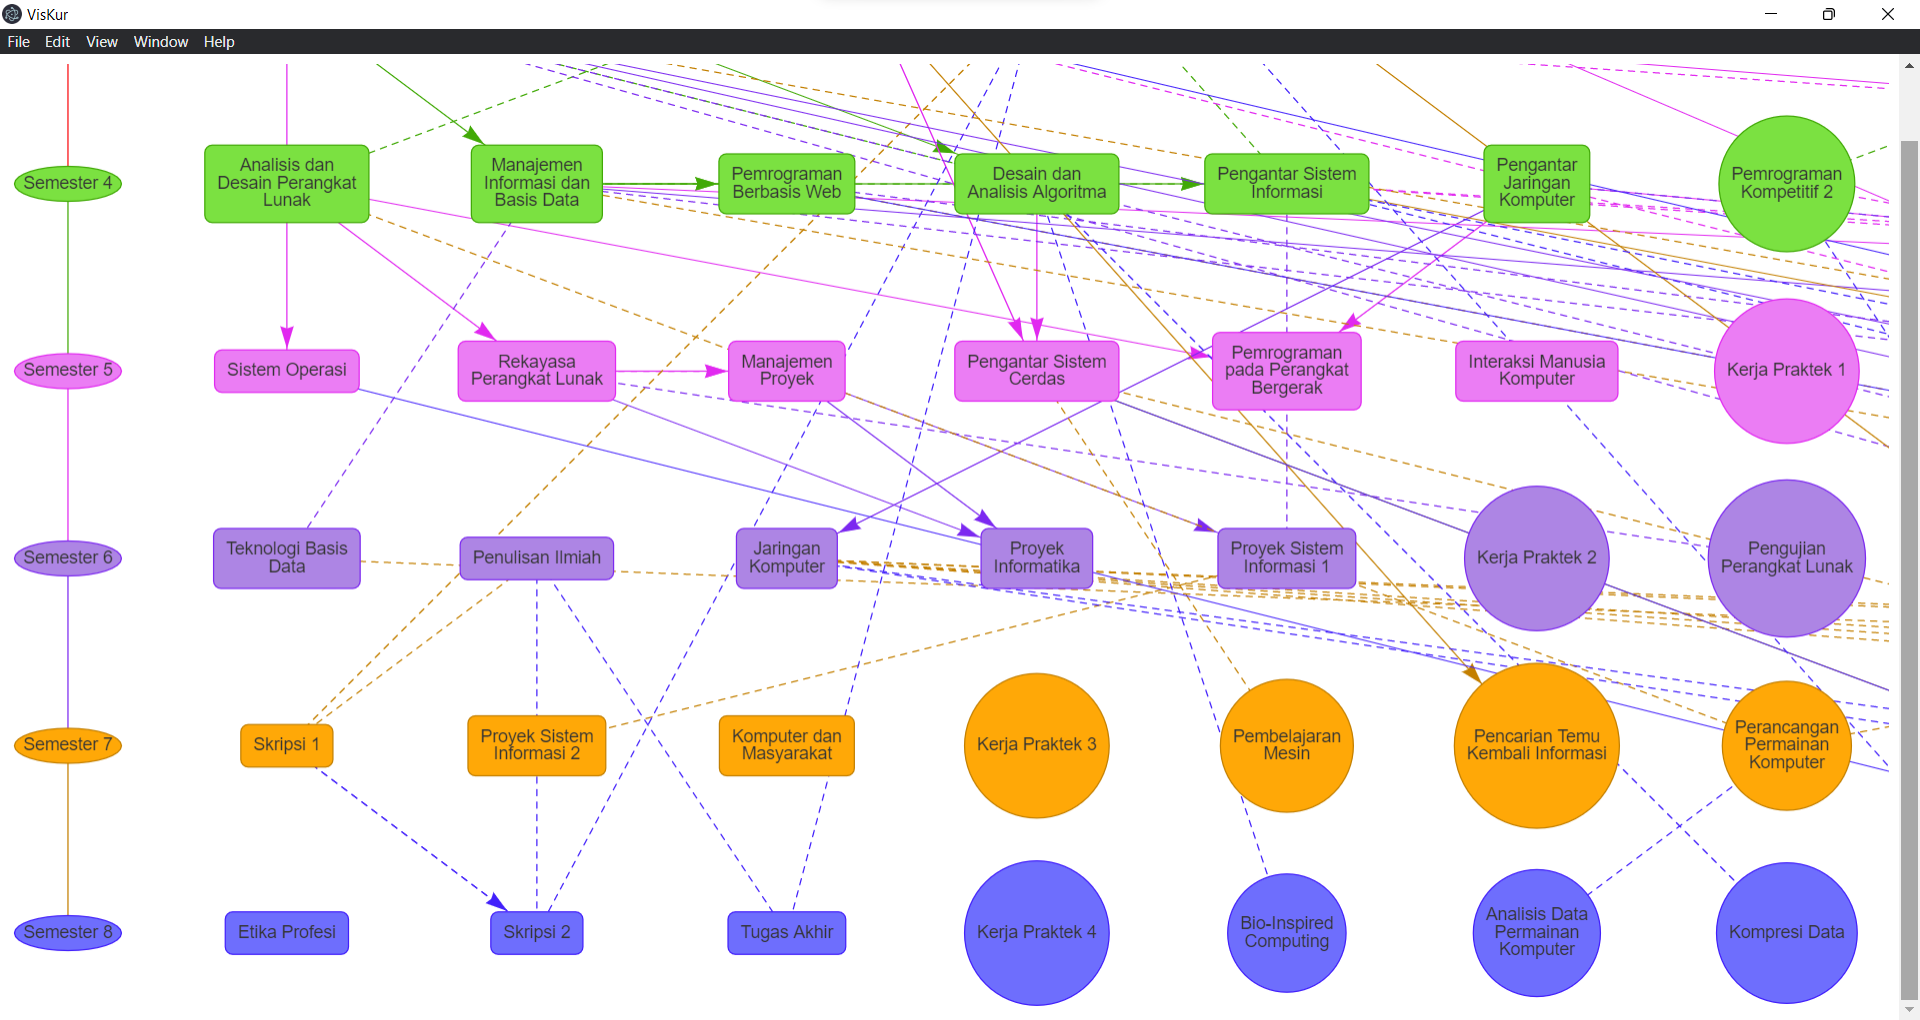
\includegraphics[width=12cm, height=8cm]{Gambar/Network2.png}
        \caption{Hasil visualisasi \textit{Network}2}
        \label{fig:gambarNetwork2}
    \end{figure}
    
    \item Contoh hasil visualisasi \textit{Timeline} dapat dilihat pada Gambar \ref{fig:gambarTimeline1} dan Gambar \ref{fig:gambarTimeline2}.
    
    \begin{figure}[H]
        \centering
        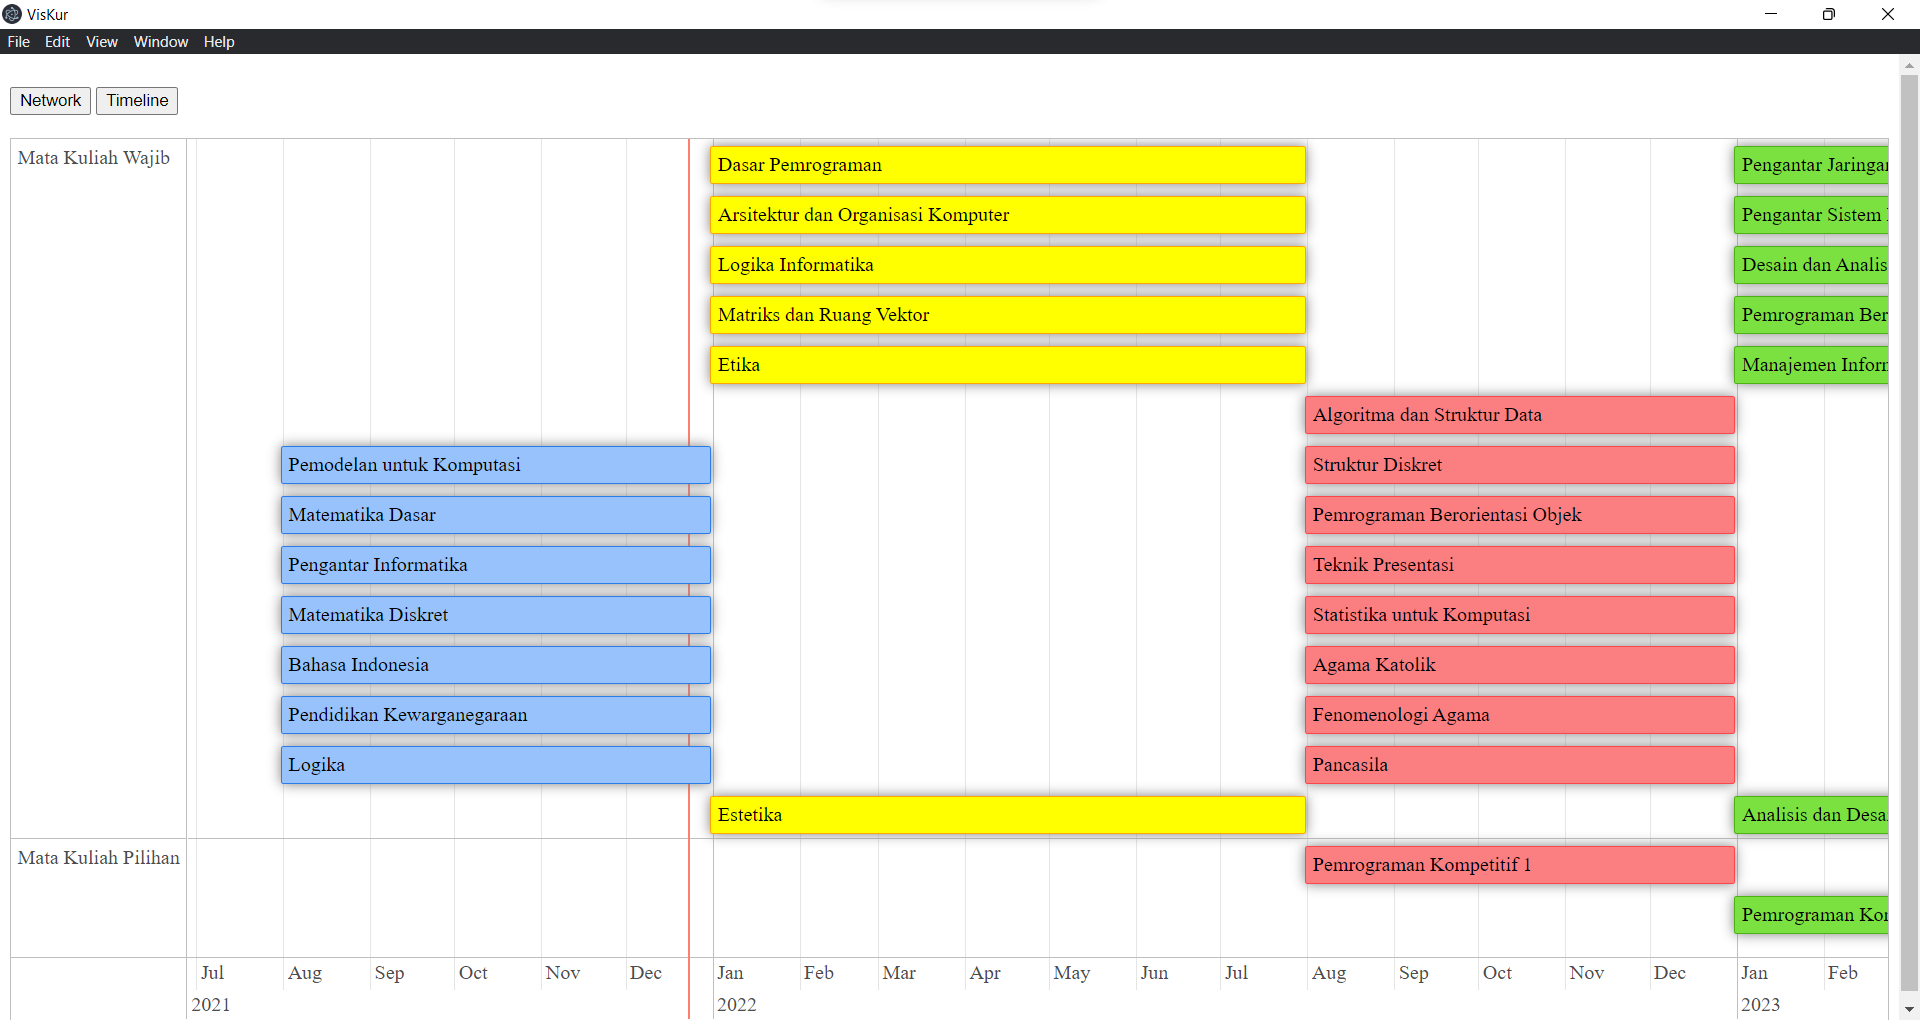
\includegraphics[width=12cm, height=8cm]{Gambar/Timeline1.png}
        \caption{Hasil visualisasi \textit{Timeline}1}
        \label{fig:gambarTimeline1}
    \end{figure}
    
    \begin{figure}[H]
        \centering
        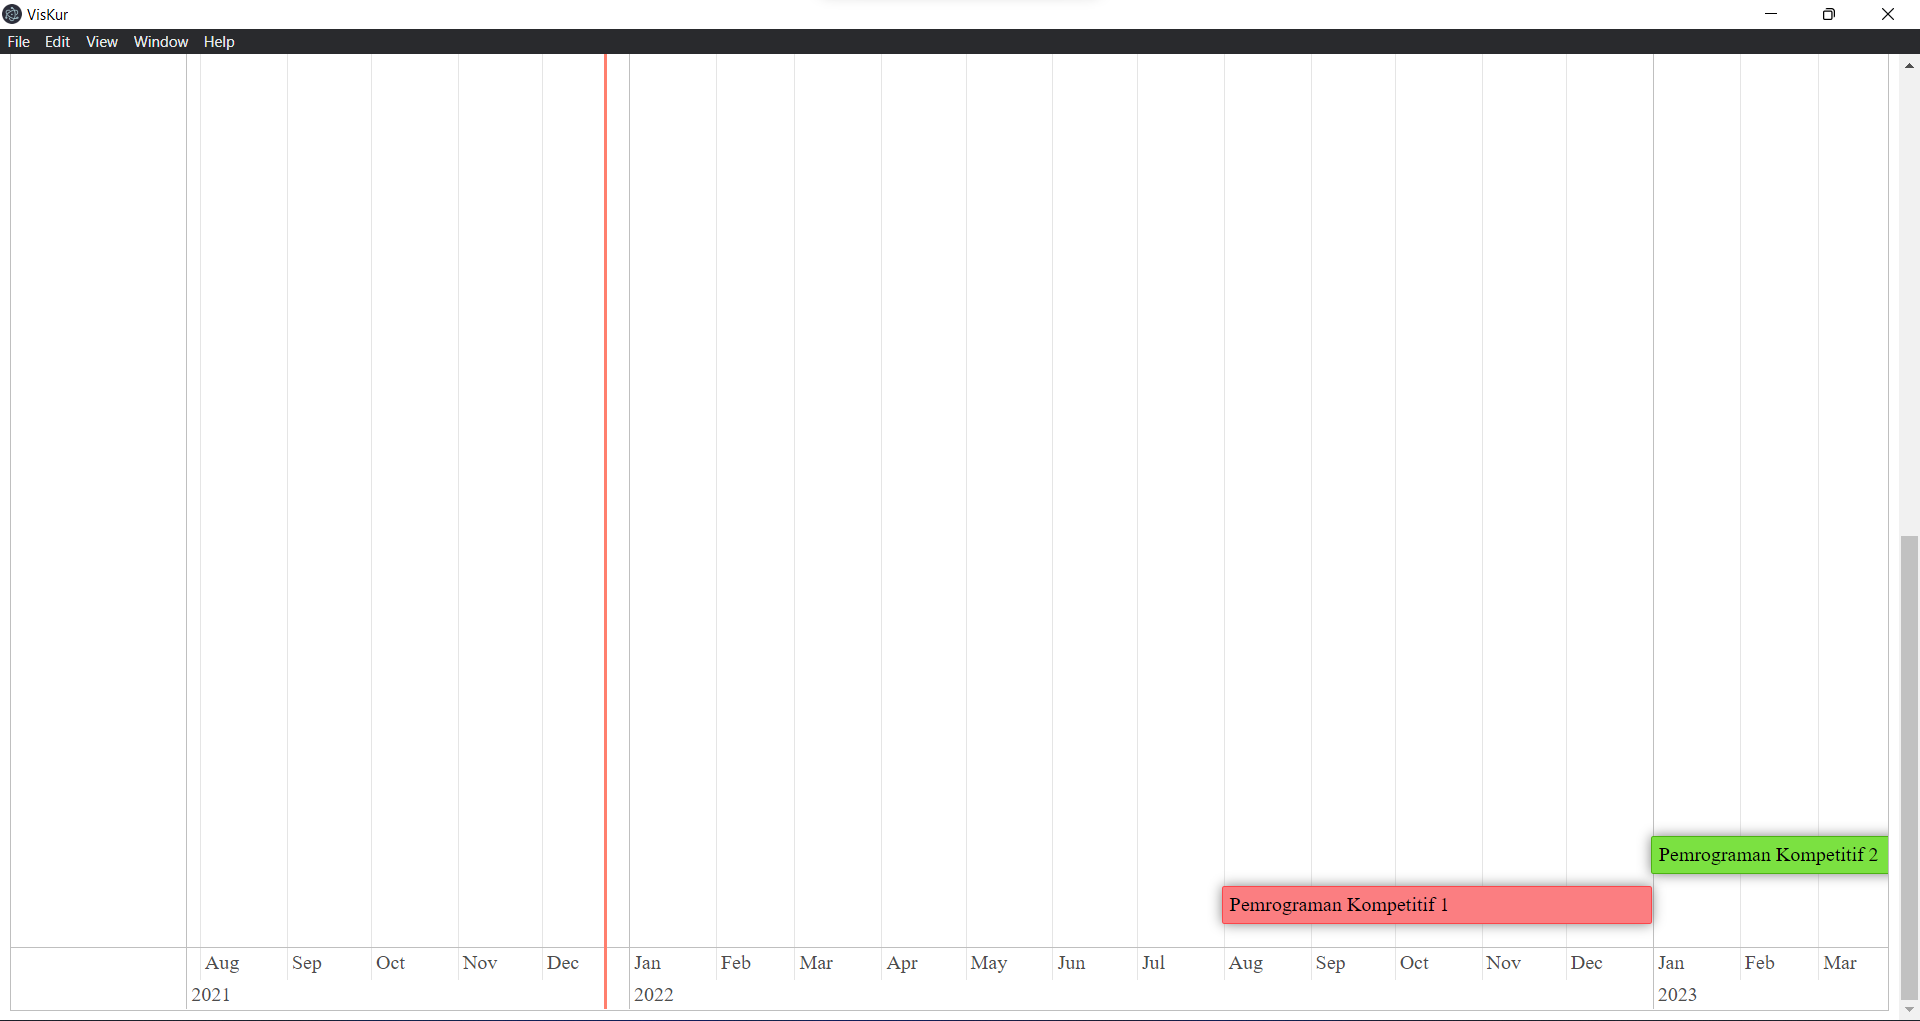
\includegraphics[width=12cm, height=8cm]{Gambar/Timeline2.png}
        \caption{Hasil visualisasi \textit{Timeline}2}
        \label{fig:gambarTimeline2}
    \end{figure}
    
\end{itemize}

\section{Pengujian}

\subsection{Pengujian Fungsional}
Pengujian fungsional dilakukan untuk mengetahui keberhasilan pemasangan perangkat lunak di komputer penulis dengan spesifikasi seperti berikut :
\vspace{3mm}

\begin{enumerate}
    \item \textit{Processor}: Intel Core i7-9750H
    \item \textit{Random Access Memory} (RAM): 16GB DDR4
    \item \textit{Graphics Processing Unit} (GPU): NVIDIA GeForce GTX 1650
    \item Sistem Operasi: Windows 11 
    \item Resolusi Layar: 1920 x 1080
\end{enumerate}

\vspace{3mm}
Berikut merupakan langkah - langkah yang dilakukan untuk memasang aplikasi VisKur:
\vspace{4mm}
\begin{itemize}
    \item Jalankan aplikasi Visualisasi-Kurikulum Setup 1.0.0.exe, maka akan muncul seperti gambar \ref{fig:gambarExe1}. Kemudian pilih apakah aplikasi dapat digunakan untuk semua pengguna atau hanya untuk saya.
    
    \begin{figure}[H]
        \centering
        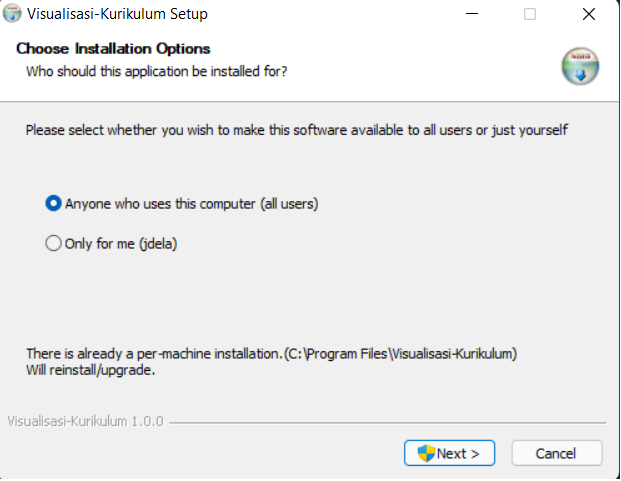
\includegraphics[width=11cm, height=8cm]{Gambar/exe1.png}
        \caption{\textit{Setup }aplikasi VisKur}
        \label{fig:gambarExe1}
    \end{figure}
    
    \item Pilih \textit{folder} tujuan untuk tempat penyimpanan aplikasi seperti pada Gambar \ref{fig:gambarExe2}, kemudian klik tombol \textit{install} untuk memasang aplikasi.
    
     \begin{figure}[H]
        \centering
        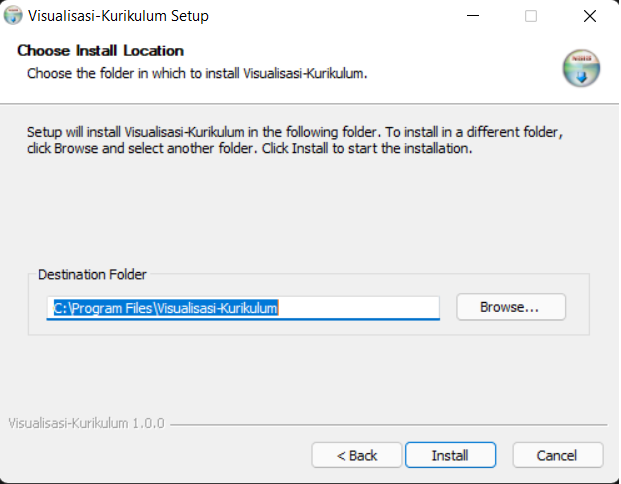
\includegraphics[width=11cm, height=8cm]{Gambar/exe2.png}
        \caption{\textit{Setup }aplikasi VisKur}
        \label{fig:gambarExe2}
    \end{figure}
    
    \item Setelah aplikasi berhasil dipasang, maka akan keluar seperti pada Gambar \ref{fig:gambarExe3}, kemudian klik tombol \textit{Finish} dan aplikasi akan langsung dijalankan.
    
    \begin{figure}[H]
        \centering
        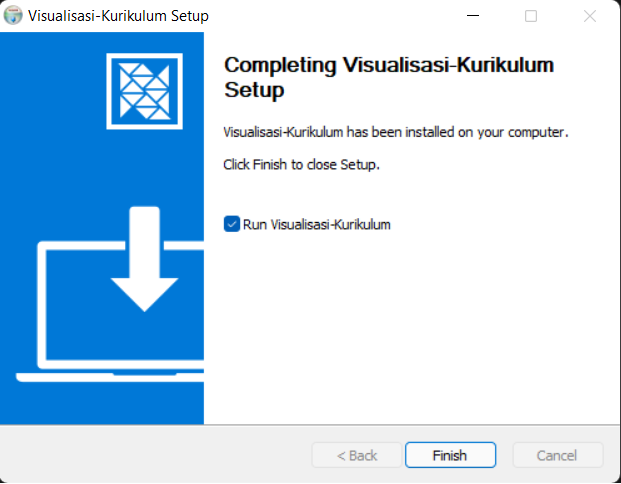
\includegraphics[width=11cm, height=8cm]{Gambar/exe3.png}
        \caption{\textit{Setup }aplikasi VisKur}
        \label{fig:gambarExe3}
    \end{figure}
    
\end{itemize}

\subsection{Pengujian Ekperimental}
\label{pengujianEksperimental}

Pengujian eksperimental pada skripsi ini akan dilakukan dengan melakukan survei kepada sepuluh orang mahasiswa aktif Universitas Katolik Parahyangan jurusan informatika yang kemudian didapatkan hasil seperti berikut:

\begin{itemize}
    \item Hasil diagram batang pada Gambar \ref{fig:gambarSurvei1} menunjukkan bahwa sembilan orang satu orang memilih tidak setuju, tiga orang memilih biasa saja, empat orang memilih setuju, dan dua orang memilih sangat setuju bahwa lebih mudah dimengerti daripada pohon kurikulum.
    
    \begin{figure}[H]
        \centering
        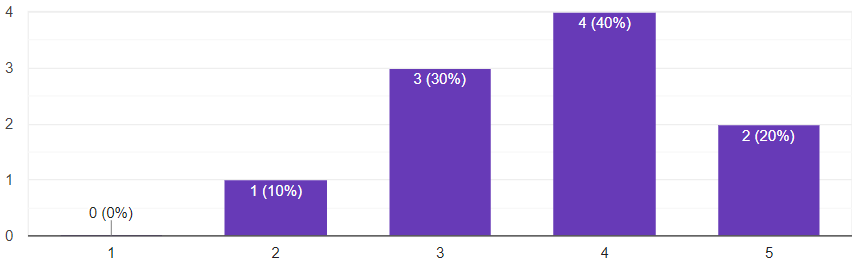
\includegraphics[width=12cm, height=5cm]{Gambar/survei1.png}
        \caption{Diagram batang hasil pemilihan aplikasi VisKur terhadap pohon kurikulum}
        \label{fig:gambarSurvei1}
    \end{figure}
    
    \item Hasil diagram lingkaran pada Gambar \ref{fig:gambarSurvei2} menunjukkan bahwa tujuh puluh persen mahasiswa memilih sangat setuju dan tiga puluh persen mahasiswa memilih sangat tidak setuju bahwa informasi yang ditampilkan oleh aplikasi VisKur lebih terpakai untuk membantu memilih mata kuliah yang akan diambil pada semester berikutnya dibandingkan dengan informasi yang ditampilkan pada pohon kurikulum. Untuk informasi yang tidak ditampilkan pada aplikasi VisKur adalah jumlah sks untuk setiap mata kuliahnya, sedangkan informasi yang tidak ada pada pohon kurikulum adalah mata kuliah pilihan.
    
    \begin{figure}[H]
        \centering
        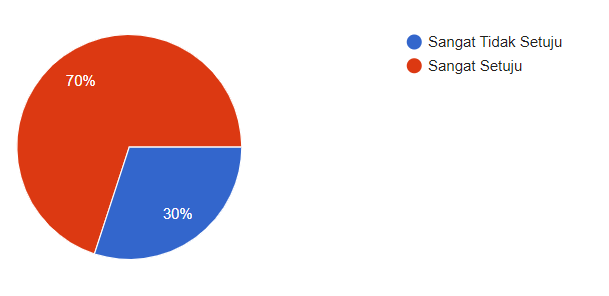
\includegraphics[width=12cm, height=6cm]{Gambar/survei2.png}
        \caption{Diagram lingkaran pemilihan aplikasi VisKur terhadap Pohon kurikulum}
        \label{fig:gambarSurvei2}
    \end{figure}
    
    \item Untuk kelebihan pohon kurikulum, menurut mereka adalah mata kuliah yang disajikan lebih jelas dan lengkap informasinya karena memiliki jumlah sks untuk setiap mata kuliahnya.
    
    \item Untuk kekurangan pohon kurikulum, menurut mereka adalah panah yang membingungkan karena warna dari setiap panahnya sama semua dan bertumpuk - tumpuk sehingga agak susah untuk memahami alurnya. Kemudian tidak adanya informasi mata kuliah pilihan serta desain yang kurang menarik atau tidak interaktif.
    
    \item Untuk kelebihan aplikasi VisKur, menurut mereka adalah penampilannya lebih menarik karena pemberian warna dan bentuk yang berbeda membantu mereka dalam membaca kurikulum. Alur hubungan antar mata kuliahnya lebih jelas sehingga lebih mudah untuk melihat prasyaratnya untuk setiap mata kuliah yang ada.
    
    \item Untuk kekurangan aplikasi Viskur, menurut mereka adalah informasi yang ditampilkan tidak selengakap informasi yang ditampilkan pada pohon kurikulum karena tidak ada jumlah sks untuk setiap mata kuliahnya.
    
    \item Hasil dari diagram lingkaran pada Gambar \ref{fig:gambarSurvei3} menunjukkan bahwa delapan puluh persen mahasiswa memilih jenis visualisasi \textit{Network} dan dua puluh persen mahasiswa memilih jenih visualisasi \textit{Timeline} yang lebih cocok untuk memvisualisasikan kurikulum 2018.
    
    \begin{figure}[H]
        \centering
        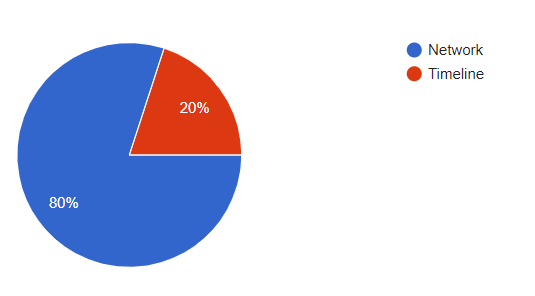
\includegraphics[width=12cm, height=6.5cm]{Gambar/survei3.png}
        \caption{\textit{Setup }aplikasi VisKur}
        \label{fig:gambarSurvei3}
    \end{figure}
    
    \item Alasan mereka lebih memilih bentuk visualisasi \textit{Network} adalah karena penampilannya lebih menarik, lebih mudah dipahami, lebih terlihat hubungannya, serta lebih interaktif karena dapat digerakan sesuai dengan kebutuhan. 
    
\end{itemize}